%!TEX root = ../NCVC3.tex

\mysection{Gコードの生成}

\vspace*{1zh}
 準備が整えば,\menu{ファイル>NCデータの生成>旋盤データの生成} を選択し,OKボタンを押すと,図11のようなシミュレーション結果が表示されます.
カスタムヘッダーに旋盤用のソリッド情報(LatheView=〇〇, 〇〇, 〇〇)が埋め込まれているので,生成後即ソリッド表示が可能です.

%\begin{figure}[H]
%\centering
%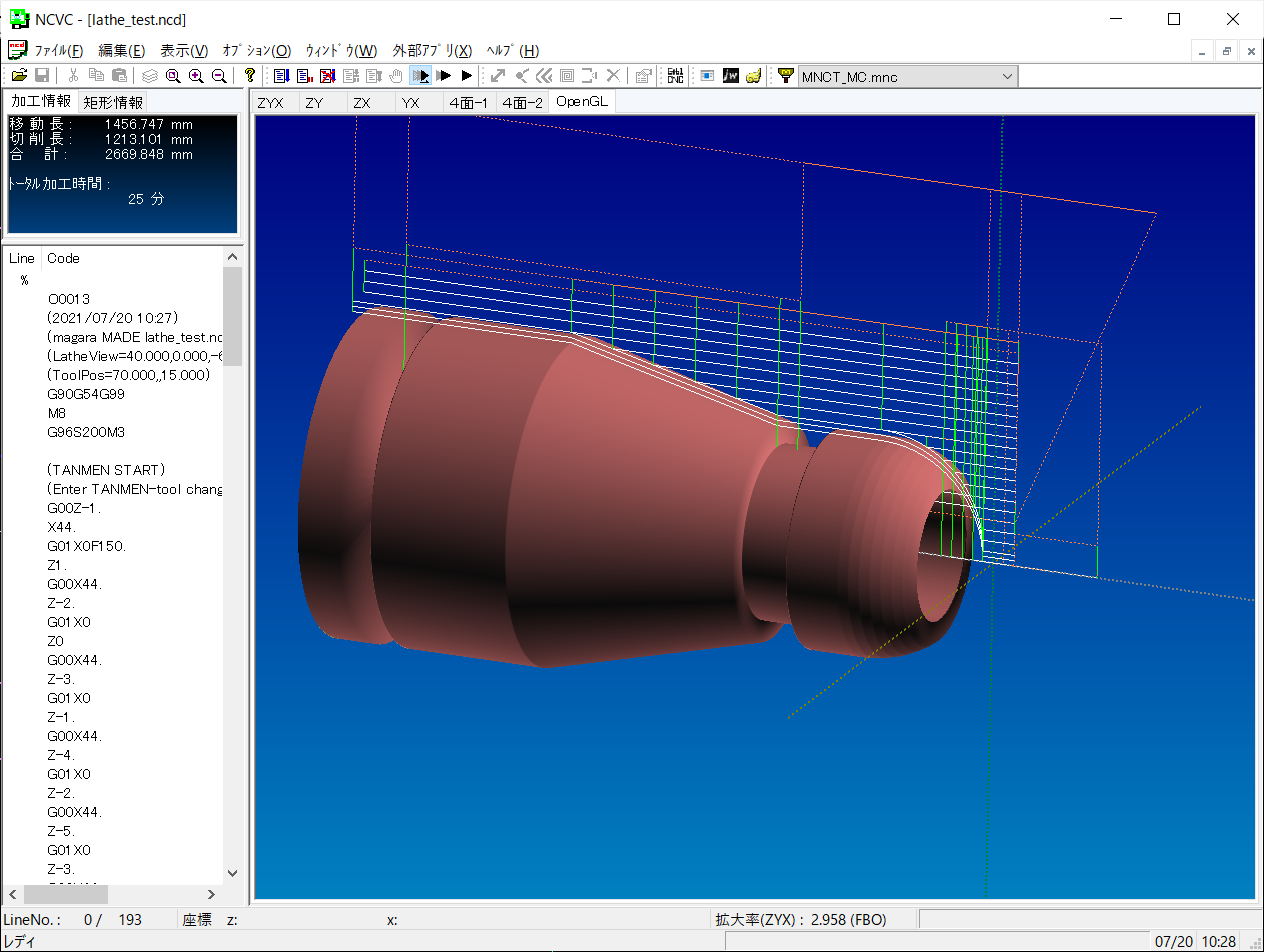
\includegraphics[scale=0.5]{No3/fig/simu1.png}
%\caption{旋盤データのシミュレーション画面Ⅰ}
%\label{fig:simu1.png}
%\end{figure}

 図11の画面でCtrl+左ダブルクリックすると,図12のようなカットモデルの表示も可能です.
内径パスの確認にご活用してください.

%\begin{figure}[H]
%\centering
%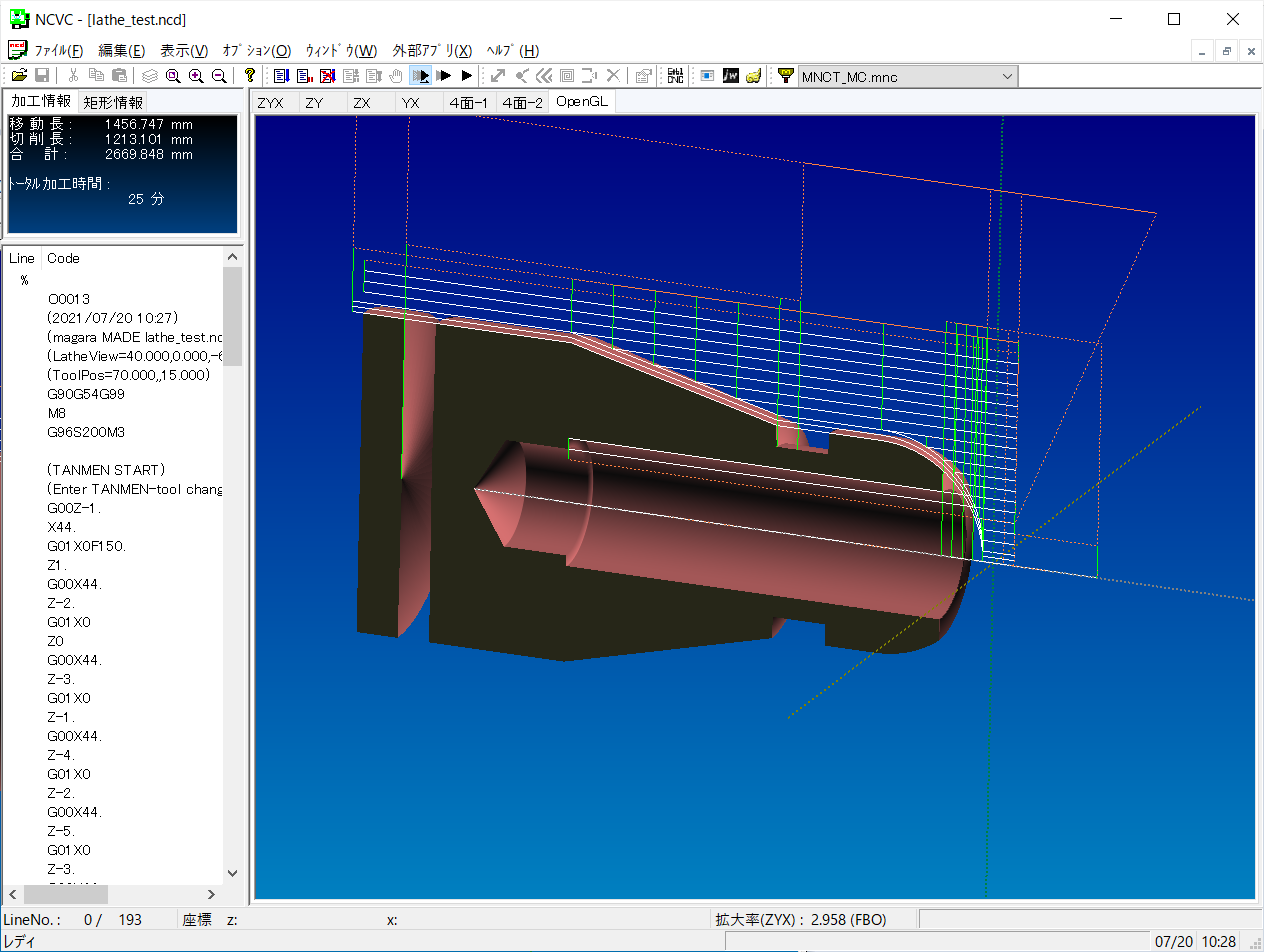
\includegraphics[scale=0.5]{No3/fig/simu2.png}
%\caption{旋盤データのシミュレーション画面Ⅱ}
%\label{fig:simu2.png}
%\end{figure}

\vspace*{3zh}
\begin{itembox}[l]{ここまでの【まとめ】}
(1) CADでの作図
\begin{itemize}
\item 工具初期位置を示す円を原点レイヤに作図
\item 端面と被削材外径を示す直線も原点レイヤに作図
\item 端面の一番下がワーク座標原点になる
\item 切削したい形状を切削レイヤに作図
\item 内径を示す形状には切削レイヤ名にINSIDEを追加
\item 溝加工や切り落としには切削レイヤ名にGROOVEを追加
\end{itemize}
(2) 加工条件とシミュレーション
\begin{itemize}
\item 旋盤用の加工条件ncjで設定する
\item カスタムヘッダーが適切に設定されていると,生成後即ソリッド表示が可能
\end{itemize}
\end{itembox}
